\documentclass[11pt]{article}

% -----------------------------
% Packages
% -----------------------------
\usepackage[a4paper,margin=1in]{geometry}
\usepackage{microtype}
\usepackage{amsmath,amssymb,bm}
\usepackage{mathtools}
\usepackage{booktabs}
\usepackage{hyperref}
\usepackage{cleveref}
\usepackage{graphicx}
\usepackage{enumitem}
\usepackage{algorithm}
\usepackage{algpseudocode}
\usepackage{listings}
\usepackage{xcolor}
\usepackage{tikz}
\usepackage{float}
\usepackage[colorinlistoftodos]{todonotes}
\usetikzlibrary{arrows.meta,positioning,shapes.geometric}

% -----------------------------
% Hyperref
% -----------------------------
\hypersetup{
  colorlinks=true,
  linkcolor=blue,
  urlcolor=blue,
  citecolor=blue
}

% -----------------------------
% Listings (Julia)
% -----------------------------
\definecolor{codebg}{RGB}{248,248,248}
\definecolor{codekw}{RGB}{0,92,173}
\definecolor{codecm}{RGB}{90,90,90}
\definecolor{codestr}{RGB}{163,21,21}

\lstdefinelanguage{Julia}{
  morekeywords={mutable,struct,function,end,return,import,Base,for,if,else,elseif,while,break,continue,in,nothing,true,false},
  sensitive=true,
  morecomment=[l]{\#},
  morestring=[b]"
}

\lstset{
  language=Julia,
  basicstyle=\ttfamily\small,
  backgroundcolor=\color{codebg},
  frame=single,
  rulecolor=\color{black!15},
  frameround=tttt,
  tabsize=2,
  showstringspaces=false,
  breaklines=true,
  breakatwhitespace=true,
  keywordstyle=\color{codekw}\bfseries,
  commentstyle=\color{codecm}\itshape,
  stringstyle=\color{codestr},
  numbers=left,
  numberstyle=\tiny\color{black!45},
  numbersep=8pt,
  xleftmargin=2.2em,
  framexleftmargin=1.8em
}

\lstset{
  extendedchars=true,
  literate={∉}{{$\notin$}}1 {∈}{{$\in$}}1 
}
% -----------------------------
% Title
% -----------------------------
\begin{document}
\begin{titlepage}
    \centering
    \includegraphics[width=0.7\textwidth]{NUS.png}
    \vspace*{0.2cm}
    
    {\huge \textbf{From Scratch: Reverse-Mode Automatic Differentiation and Integrated Gradients for Interpretability in Neural and Physics-Based Models} \par}
    
    \vspace{1.0cm}
    
    {\large \textbf{Course code: EE5311 Differentiable and Probabilistic Computing} \par}
    {\large Electrical and Computer Engineering \par}
    
    \vspace{1.0cm}
    
    {\large \textbf{Supervised By:} Prof. CHITRE, Mandar Anil \par}
    
    \vspace{1.0cm}
    
    {\large \textbf{Written By:} \par}
    {\large Liu Fei (A0275104M) \par}
    {\large Cao Yuan (A0275177U) \par}
    {\large Jin Xuan (A0328457U) \par}
    {\large Gao Jiaxuan (A0332428H) \par}
    {\large Nan Jinyao (A0319482X) \par}
    
    \vspace{0.8cm}
    
    {\large Date Last Edited: Feb 13, 2025 \par}
    
    \vfill
    
    \noindent\rule{\textwidth}{0.4pt}
    \vspace{0.1cm}
    \textbf{Declaration:} We understand what plagiarism is and have ensured We, Group 6, did not plagiarise for this assignment. We declare that our submission for CA1 Synthesis Essay is our own work. This assignment is in partial fulfilment of the requirements for the module EE5311.
    
    \vspace{0.2cm}
    \textbf{Declaration of AI-generated material:} During the preparation of this work, the author used generative AI tools (Google Gemini) to assist in LaTeX code generation (specifically for TikZ diagrams) and linguistic polishing. The author has reviewed and edited the content as needed and takes full responsibility for the content of the publication.
    \noindent\rule{\textwidth}{0.4pt}
\end{titlepage}

\begin{abstract}
This work presents a lightweight, ground-up implementation of a reverse-mode automatic differentiation (AD) engine in Julia. Centered on a Tensor abstraction, the framework leverages operator overloading and closure-based pullbacks to compute Vector-Jacobian Products (VJPs) across dynamic computational graphs, with DFS-based topological sorting ensuring robust gradient scheduling. Beyond core AD, we implement Integrated Gradients (IG) to provide equitable feature attribution for both deep learning and differentiable physical simulations. The resulting pipeline demonstrates a unified approach to sensitivity and attribution analysis, effectively bridging the gap between low-level differentiable primitives and high-level interpretability in scientific computing. Our source code is open-source and available at: \url{https://github.com/nanjinyao/EE5311_CA1_AD_IG}
\end{abstract}


\section{Introduction}

Interpretability is critical not only for deep learning but also for physical systems governed by differentiable laws. To bridge these domains, this work presents a lightweight reverse-mode automatic differentiation (AD) engine implemented from first principles in Julia~\cite{bezanson2017julia}.

The framework is centered on a \texttt{Tensor} abstraction that dynamically constructs computational graphs via operator overloading. By utilizing closure-based \textit{pullbacks} and Depth-First Search (DFS) topological scheduling, the engine efficiently computes Vector-Jacobian Products (VJPs) without the overhead of explicit Jacobian matrices.

Building on this foundation, we integrate \textit{Integrated Gradients} (IG) as a unified attribution mechanism. Experiments on differentiable physical simulations (e.g., projectile motion) demonstrate that this pipeline effectively quantifies parameter sensitivity. This approach highlights how gradients serve as a universal language, connecting low-level differentiable primitives to high-level physical reasoning.

\section{Core Principle: Chain Rule and VJP}
The mathematical foundation of reverse-mode AD is the \textbf{Chain Rule} for multi-variable composite functions. In a computational graph, if a scalar output $L$ (usually the loss) depends on a node $u$ through several downstream nodes $v_i$, the gradient of $L$ with respect to $u$ is given by the sum of contributions from all paths:
\begin{equation}
\frac{\partial L}{\partial u} = \sum_{i} \frac{\partial L}{\partial v_i} \frac{\partial v_i}{\partial u}
\end{equation}

In our implementation, we do not explicitly construct large Jacobian matrices. Instead, we compute the \textbf{Vector-Jacobian Product (VJP)}. 
\begin{itemize}[leftmargin=1.5em]
    \item \textbf{Forward Pass:} Compute and store the output $v = f(u)$.
    \item \textbf{Backward Pass:} Receive the downstream gradient $\nabla_v L$, multiply it by the local derivative $\frac{\partial v}{\partial u}$, and \textbf{accumulate} it into the gradient of $u$.
\end{itemize}
The accumulation (\texttt{.+=}) is crucial: if a variable is used in multiple operations (fan-out $> 1$), its total gradient must be the sum of gradients from all its consumers.

\section{Core Abstraction: The \texttt{Tensor} Struct}
The engine is built around a mutable \texttt{Tensor} object. Each \texttt{Tensor} acts as a node in a dynamic computational graph, aware of its data, its gradient, and its ancestors.

\begin{lstlisting}[language=Julia, caption={The actual Tensor implementation from ad\_v7.ipynb}]
mutable struct Tensor
    data::Array{Float64}          # Numerical values
    grad::Array{Float64}          # Accumulated gradients
    _backward::Function           # Pullback closure
    _prev::Set{Tensor}            # Parent nodes for graph traversal
    op::String                    # Debugging label
    requires_grad::Bool           # Gradient tracking flag

    function Tensor(data; _children=(), _op="", requires_grad=true)
        if data isa Number
            d = reshape([Float64(data)], 1, 1)
        else
            arr = convert(Array{Float64}, data)
            d = ndims(arr) == 1 ? reshape(arr, :, 1) : arr
        end
        g = zeros(size(d))
        # Structural pruning: only track parents if grad is required
        prev = requires_grad ? Set{Tensor}(_children) : Set{Tensor}()
        new(d, g, () -> nothing, prev, _op, requires_grad)
    end
end
\end{lstlisting}

The most critical design choice is the \texttt{\_backward} field. It is a \textbf{closure} that captures the context of the forward operation (like the values of the operands), allowing the local backpropagation logic to be encapsulated within the node itself.

\section{Algorithm Flow: Construction and Backtracking}
The execution of the AD engine consists of two distinct phases:

\subsection{Phase 1: Dynamic Graph Construction via Operator Overloading}

To visualize the complete workflow, Figure \ref{fig:ad_flowchart} illustrates the transition from the forward construction to the backward accumulation.

\begin{figure}[htbp]
\centering
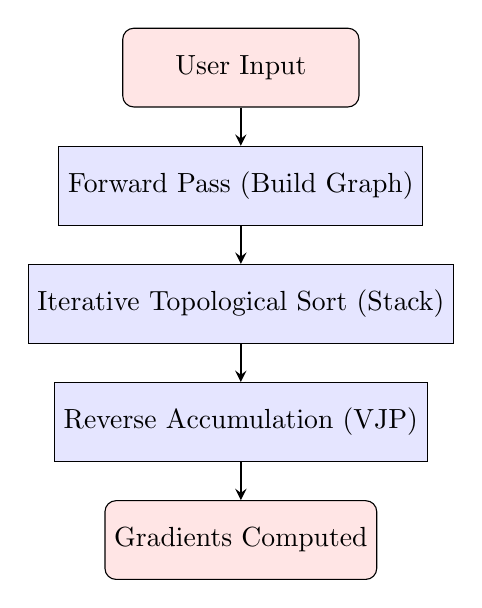
\begin{tikzpicture}[
    node distance=1.5cm,
    startstop/.style={rectangle, rounded corners, minimum width=3cm, minimum height=1cm,text centered, draw=black, fill=red!10},
    process/.style={rectangle, minimum width=3cm, minimum height=1cm, text centered, draw=black, fill=blue!10},
    decision/.style={diamond, minimum width=3cm, minimum height=1cm, text centered, draw=black, fill=green!10},
    arrow/.style={thick,->,>=stealth}
]

\node (start) [startstop] {User Input};
\node (forward) [process, below of=start] {Forward Pass (Build Graph)};
\node (topo) [process, below of=forward] {Iterative Topological Sort (Stack)};
\node (backward) [process, below of=topo] {Reverse Accumulation (VJP)};
\node (end) [startstop, below of=backward] {Gradients Computed};

\draw [arrow] (start) -- (forward);
\draw [arrow] (forward) -- (topo);
\draw [arrow] (topo) -- (backward);
\draw [arrow] (backward) -- (end);

\end{tikzpicture}
\caption{Flowchart of the Reverse-Mode Automatic Differentiation Engine.}
\label{fig:ad_flowchart}
\end{figure}

In our engine, the forward pass does more than just compute values; it builds a directed acyclic graph (DAG) in real-time. When an operation like \texttt{a * b} is invoked, the engine intercepts it via operator overloading to "plant the seeds" for the backward pass. For matrix-based multiplication, the process follows three core steps:

\begin{enumerate}[leftmargin=1.5em]
    \item \textbf{Forward Pass:} Compute the product $\mathbf{C} = \mathbf{A}\mathbf{B}$. To ensure a uniform interface, our implementation treats even scalars as $1 \times 1$ matrices and vectors as $n \times 1$ column matrices.
    \item \textbf{Structural Pruning:} A new \texttt{Tensor} node is created. To optimize memory and computation, its \texttt{\_prev} set is populated only by parent nodes that have \texttt{requires\_grad = true}. If neither parent requires a gradient, the child node's tracking is disabled as well.
    \item \textbf{VJP (Pullback) Definition:} The engine attaches a closure that implements the Vector-Jacobian Product for matrix multiplication. Given the gradient of the loss with respect to the output $\mathbf{G} = \frac{\partial L}{\partial \mathbf{C}}$, the gradients for the inputs are computed using the following transpose rules:
    \begin{equation}
    \frac{\partial L}{\partial \mathbf{A}} = \mathbf{G}\mathbf{B}^\top, \quad \frac{\partial L}{\partial \mathbf{B}} = \mathbf{A}^\top\mathbf{G}
    \end{equation}
\end{enumerate}



\begin{lstlisting}[language=Julia, caption={Matrix Multiplication implementation with VJP logic from ad\_v7.ipynb}]
function *(a::Tensor, b::Tensor)
    # Determine if the output needs to track gradients
    out_rg = a.requires_grad || b.requires_grad
    # Structural Pruning: Only track parents that participate in backprop
    kids = filter(x -> x.requires_grad, (a, b)) 
    
    # Perform forward matrix multiplication
    out = Tensor(a.data * b.data, _children=kids, _op="MatMul", requires_grad=out_rg)
    
    if out_rg
        function _backward()
            # Matrix VJP: dL/dA = (dL/dC) * B' and dL/dB = A' * (dL/dC)
            # .+= ensures gradients from different paths are accumulated
            if a.requires_grad 
                a.grad .+= out.grad * transpose(b.data) 
            end
            if b.requires_grad 
                b.grad .+= transpose(a.data) * out.grad 
            end
        end
        out._backward = _backward
    end
    return out
end
\end{lstlisting}

\subsection{Phase 2: Reverse Scheduling via Iterative Topological Sort}

To ensure gradients are propagated correctly, a node must only be processed after all its downstream consumers have finished accumulating their gradients. While a recursive DFS is intuitive, it can lead to \textbf{stack overflow} in deep computational graphs. Our implementation utilizes an \textbf{iterative DFS} with an explicit stack to generate the topological order, ensuring both memory stability and execution correctness.

\paragraph{The Iterative DFS Mechanism:}
The algorithm uses a stack to manage the traversal, where each entry is a tuple \texttt{(node, processed\_flag)}:
\begin{itemize}[leftmargin=1.5em]
    \item \textbf{Discovery Phase:} When a node is first encountered (\texttt{processed\_flag = false}), it is pushed back onto the stack with the flag set to \texttt{true}, followed by all its unvisited parents.
    \item \textbf{Post-order Completion:} When a node is popped and its flag is \texttt{true}, it means all its dependencies have been explored. The node is then added to the \texttt{topo} list. This effectively simulates post-order traversal without recursion.
    \item \textbf{Reversal:} Reversing this list yields a valid reverse-topological order, starting from the output and ending at the inputs.
\end{itemize}

\begin{lstlisting}[language=Julia, caption={Iterative topological sort and backward execution from ad\_v7.ipynb}]
function backward_iterative(root::Tensor; init_grad=nothing)
    # Early exit if root does not participate in gradients
    if !root.requires_grad return nothing end

    # --- Step 1: Iterative Topological Sort ---
    topo = Tensor[]
    visited = Set{Tensor}()
    stack = [(root, false)]  # (node, processed_flag)
    
    while !isempty(stack)
        curr, processed = pop!(stack)
        if curr in visited continue end
        
        if processed
            push!(visited, curr)
            push!(topo, curr) # Post-order: added after all ancestors
        else
            # Re-push current node with processed=true
            push!(stack, (curr, true))
            # Push all unvisited parents to the stack
            for parent in curr._prev
                if parent ∉ visited 
                    push!(stack, (parent, false)) 
                end
            end
        end
    end
    
    # --- Step 2: Gradient Seeding ---
    if init_grad === nothing
        root.grad .= 1.0
    else
        # Stability check: ensure dimensions match
        root.grad .= (init_grad isa Number) ? Float64(init_grad) : init_grad
    end

    # --- Step 3: Reverse-Topological Replay ---
    # Replay pullbacks in reverse order (from output to input)
    for node in reverse(topo)
        node._backward()
    end
end
\end{lstlisting}

By using a stack-based iterative approach, the engine can handle arbitrarily deep models (like very deep ResNets or long sequences in RNNs) that would otherwise crash a recursive implementation. The \texttt{reverse(topo)} loop ensures that when \texttt{node.\_backward()} is executed, the \texttt{node.grad} field is "fully baked"—meaning it has already received all partial gradient contributions from every downstream operation (see Algorithm~\ref{alg:reverse-ad}).

\section{Integrated Gradients for Interpretability}

While raw gradients provide local sensitivity, they often suffer from the \textit{saturation problem} in deep networks or complex physical models, where the gradient becomes near-zero even for important features. To address this, we implement \textbf{Integrated Gradients (IG)}, which computes attribution by integrating the gradients along a straight-line path from a baseline $x_0$ to the input $x$. The continuous definition for the $i$-th feature is:
\begin{equation}
\mathrm{IG}_i(x) \coloneqq (x_i - x_{0,i}) \int_{\alpha=0}^{1} \frac{\partial F(x_0 + \alpha(x - x_0))}{\partial x_i} d\alpha
\end{equation}
As analytical integration is typically intractable for complex differentiable models $F$, we approximate this integral using a \textbf{Riemann sum}. By sampling gradients at $m$ discrete points along the path and averaging them, we obtain the computable discrete form used in our implementation (Algorithm~\ref{alg:ig-ad}):
\begin{equation}
\mathrm{IG}_i(x) \approx (x_i - x_{0,i}) \times \frac{1}{m} \sum_{k=1}^{m} \nabla_x F\left(x_0 + \frac{k}{m}(x - x_0)\right)
\end{equation}

\subsection{Key Implementation Details}
Our implementation in Julia is designed to be versatile, supporting both neural networks (via \texttt{Chain}) and arbitrary physical functions. Key features include:
\begin{itemize}[leftmargin=1.5em]
    \item \textbf{Dual Mode Support:} The method can compute gradients using our \texttt{:ad} engine or via \texttt{:fd} (Finite Differences) for non-differentiable black-box functions.
    \item \textbf{Gradient Resetting:} To avoid accumulation of gradients from previous interpolation steps, we explicitly reset \texttt{xt.grad}, \texttt{out.grad}, and \texttt{y.grad} to zero in each iteration.
    \item \textbf{Dimensional Alignment:} Inputs and baselines are normalized to 2D arrays to ensure matrix operations remain consistent.
\end{itemize}

\begin{lstlisting}[language=Julia, caption={Integrated Gradients implementation from ad\_v7.ipynb}]
function integrated_gradients(model,
    input,
    baseline;
    steps::Int=50,
    target::Union{Nothing,Int}=nothing,
    method::Symbol=:ad,
    fd_eps::Float64=1e-5)

    # Normalize input/baseline to 2D arrays (n x 1)
    x = input isa Number ? reshape([Float64(input)], 1, 1) : convert(Array{Float64}, input)
    x0 = baseline isa Number ? reshape([Float64(baseline)], 1, 1) : convert(Array{Float64}, baseline)

    @assert size(x) == size(x0) "input and baseline must have same shape"

    diff = x .- x0  # Direction vector from baseline to input
    total_grads = zeros(size(x))

    # Riemann approximation of path integral
    for s in 1:steps
        alpha = s / steps  # Interpolation factor
        z = x0 .+ alpha .* diff  # Interpolated point on the path

        if method == :ad
            # Automatic differentiation approach
            xt = Tensor(z, _op="Input")
            out = model(xt)
            # Use helper to ensure a scalar output for backpropagation
            y = to_scalar(out; target=target)

            # Reset gradients before backward pass to avoid step pollution
            if model isa Chain
                zero_grad!(model)
            end
            xt.grad .= 0.0
            out.grad .= 0.0
            y.grad .= 0.0

            backward(y)
            total_grads .+= xt.grad

        elseif method == :fd
            # Finite difference approach for black-box models
            g, _ = grad_fd(model, copy(z); eps=fd_eps)
            total_grads .+= g

        else
            error("Unknown method: $method. Use :ad or :fd.")
        end
    end

    # Compute final attributions: (input - baseline) * average_gradient
    avg_grads = total_grads ./ steps
    attrs = diff .* avg_grads
    return attrs
end
\end{lstlisting}

\subsection{Completeness and Attribution}
One major advantage of this implementation is that it satisfies the \textbf{Completeness Axiom}: the sum of the resulting attribution vector \texttt{attrs} will approximately equal the difference in the model's output, $F(x) - F(x_0)$. This provides a physically grounded interpretation of how much each parameter (like velocity or damping in a physical system) contributes to the final outcome.

\section{Numerical Experiments and Case Studies}
We demonstrate the efficacy of our from-scratch AD and IG implementation through two case studies: optimizing a physics-based projectile model and interpreting a neural network classifier.
These experiments validate that the engine correctly handles gradient propagation for both explicit physical equations and learned black-box functions.

\subsection{Case Study I: Physics-Based Model --- Robotic Projectile Motion}
This case study utilizes the AD engine in two distinct ways: first for parameter optimization (Gradient Descent), and second for model interpretability (Integrated Gradients).

\subsubsection{Optimization of Trajectory}
The goal is to optimize the launch velocity $v$ and angle $\theta$ of a projectile to hit a target hoop at coordinates $(4.0, 3.1)$. The loss function is defined as the squared Euclidean distance between the projectile's position at the target x-coordinate and the hoop's height:
\[ L(v, \theta) = (y_{\text{pred}}(v, \theta) - h_{\text{hoop}})^2 \]
Using our AD engine, we compute $\nabla L$ and perform gradient descent. Figure~\ref{fig:netball_traj} shows the optimization progress from an initial failing trajectory to a successful shot.

\begin{figure}[H]
    \centering
    \includegraphics[width=0.8\textwidth]{netball_optimized_en.png}
    \caption{Trajectory optimization using reverse-mode AD. The red line shows the optimized path hitting the target hoop.}
    \label{fig:netball_traj}
\end{figure}

\subsubsection{Explainability with IG}
We apply Integrated Gradients to understand the sensitivity of the final trajectory height with respect to the launch parameters. Figure~\ref{fig:netball_ig} illustrates the attribution scores, indicating which parameter (velocity or angle) had a more significant impact on the final outcome relative to the baseline.

\begin{figure}[H]
    \centering
    \includegraphics[width=0.6\textwidth]{netball_ig.png}
    \caption{Integrated Gradients attribution for the Netball model, showing the contribution of velocity and angle to the result.}
    \label{fig:netball_ig}
\end{figure}

\subsection{Case Study II: Neural Model --- Feature Importance in Iris Classification}
We train a Multi-Layer Perceptron (MLP) on the Iris dataset~\cite{fisher1936use} to demonstrate the engine's capability in a standard deep learning context. The network consists of input, hidden, and output layers with ReLU activations, trained using Cross-Entropy loss.

\subsubsection{Training Performance}
The model is trained for 100 epochs using SGD. The loss curve in Figure~\ref{fig:iris_loss} confirms the correct implementation of the backward pass through the composition of linear and non-linear layers.

\begin{figure}[H]
    \centering
    \includegraphics[width=0.6\textwidth]{iris_loss.png}
    \caption{Training loss for the MLP on the Iris dataset, validating the AD engine's stability.}
    \label{fig:iris_loss}
\end{figure}

\subsubsection{Feature Attribution}
Using IG, we analyze the importance of the four input features (Sepal/Petal Length/Width) for a specific prediction (e.g., Setosa). Figure~\ref{fig:iris_ig} highlights the most influential features driving the model's decision, providing transparency to the "black box" neural network.

\begin{figure}[H]
    \centering
    \includegraphics[width=0.6\textwidth]{iris_ig.png}
    \caption{Feature importance attribution for an Iris Setosa prediction.}
    \label{fig:iris_ig}
\end{figure}

\section{Conclusion}
This work presented a minimalist yet functional implementation of Reverse-Mode Automatic Differentiation and Integrated Gradients in Julia. By decomposing programs into computational graphs of primitive operations, we demonstrated how exact gradients can be computed efficiently. The application of this engine to both a physics-based optimization problem and a neural network classification task highlights the universality of the approach. The project serves as a pedagogical bridge between the theoretical foundations of differentiable programming and its practical application in model interpretability.

\begin{thebibliography}{9}
\bibitem{griewank2008evaluating}
Griewank, A., \& Walther, A. (2008). Evaluating derivatives: principles and techniques of algorithmic differentiation. SIAM.

\bibitem{sundararajan2017axiomatic}
Sundararajan, M., Taly, A., \& Yan, Q. (2017). Axiomatic attribution for deep networks. In International Conference on Machine Learning (pp. 3319-3328). PMLR.

\bibitem{baydin2017automatic}
Baydin, A. G., Pearlmutter, B. A., Radul, A. A., \& Siskind, J. M. (2017). Automatic differentiation in machine learning: a survey. Journal of Machine Learning Research, 18(153), 1-43.

\bibitem{bezanson2017julia}
Bezanson, J., Edelman, A., Karpinski, S., \& Shah, V. B. (2017). Julia: A fresh approach to numerical computing. SIAM review, 59(1), 65-98.

\bibitem{fisher1936use}
Fisher, R. A. (1936). The use of multiple measurements in taxonomic problems. Annals of eugenics, 7(2), 179-188.
\end{thebibliography}



\appendix
\section{Appendix}
\subsection{Algorithms} \label{app:algorithms}

\begin{algorithm}[H]
\caption{Reverse-Mode AD via Iterative Topological Sort}
\label{alg:reverse-ad}
\begin{algorithmic}[1]
\Require Output node $y$ (scalar \texttt{Tensor})
\Ensure Gradients stored in \texttt{grad} fields of all reachable nodes
\State \textbf{Phase 1: Iterative Topological Sort}
\State $\texttt{topo} \leftarrow \text{Empty List}$
\State $\texttt{visited} \leftarrow \text{Empty Set}$
\State $\texttt{stack} \leftarrow [(y, \textbf{false})]$ \Comment{Tuple: (node, processed\_flag)}
\While{$\texttt{stack}$ is not empty}
    \State $(v, \text{processed}) \leftarrow \textsc{Pop}(\texttt{stack})$
    \If{$v \notin \texttt{visited}$}
        \If{\text{processed}}
            \State $\textsc{Push}(\texttt{visited}, v)$
            \State $\textsc{Push}(\texttt{topo}, v)$ \Comment{Post-order insertion}
        \Else
            \State $\textsc{Push}(\texttt{stack}, (v, \textbf{true}))$
            \ForAll{$parent \in v.\_prev$}
                 \If{$parent \notin \texttt{visited}$}
                    \State $\textsc{Push}(\texttt{stack}, (parent, \textbf{false}))$
                 \EndIf
            \EndFor
        \EndIf
    \EndIf
\EndWhile
\State \textbf{Phase 2: Reverse Accumulation}
\State $y.\texttt{grad} \leftarrow 1$
\ForAll{$v \in \textsc{Reverse}(\texttt{topo})$}
  \State $v.\texttt{\_backward}()$ \Comment{Executes VJP closure}
\EndFor
\end{algorithmic}
\end{algorithm}

\begin{algorithm}[H]
\caption{Integrated Gradients using Reverse-Mode AD}
\label{alg:ig-ad}
\begin{algorithmic}[1]
\Require Model $F(\cdot)$, input $x$, baseline $x'$, steps $m$, optional target index
\Ensure Attribution vector $\mathrm{IG}(x)$
\State $\Delta \leftarrow x-x'$, \quad $G \leftarrow 0$
\For{$k=1$ to $m$}
  \State $\alpha \leftarrow k/m$
  \State $z \leftarrow x' + \alpha \Delta$
  \State Wrap $z$ as input \texttt{Tensor} and compute scalar output $y$
  \State \textsc{Backward}$(y)$ to obtain $\nabla_x F(z)$
  \State $G \leftarrow G + \nabla_x F(z)$
\EndFor
\State $\bar{G} \leftarrow G/m$
\State $\mathrm{IG}(x) \leftarrow \Delta \odot \bar{G}$
\end{algorithmic}
\end{algorithm}

\subsection{Member Contributions}
\begin{itemize}
    \item \textbf{Cao Yuan}: Proposed the core idea and integrated the code.
    \item \textbf{Liu Fei}: Participated in the toy example development and case optimization.
    \item \textbf{Jin Xuan}: Implemented complex main operators, conducted case verification, and wrote the paper.
    \item \textbf{Gao Jiaxuan}: Responsible for operator and method optimization.
    \item \textbf{Nan Jinyao}: Responsible for application case development, code integration, and paper writing.
\end{itemize}

\end{document}